In the last decades technology has advanced creating mesoscopic devices that are approaching dimensions of the order of nanometers.
If it is true that this techonological improvement is happening thanks to more insight on the physics of these mesoscopic structures, it is also true that better technology allows better experiments that in turn result in deepening our understanding.
There are also some cases where the theoretical study of this devices represents a better way of understanding their own physics: this is the case with Quantum dots.

Quantum dots are fabricated nanoscale structures capable to capture electrons.
In particular it is possibile to create  two-dimensional Q-dots from 2 layers of semiconductors (e.g GaAs Q-dots).
Typical dimensions are about $\SI{10}{nm}$ of thickness and few hundreds of nanometers of width.
Between the interfaces takes place a really narrow potential well that allows the formation of a quasi-two-dimensional electron gas.

\begin{figure}[H]
  \centering
  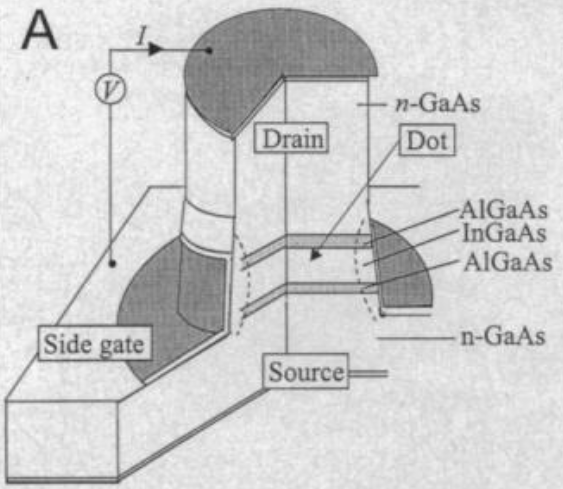
\includegraphics[width=.3\textwidth]{Images/qdotscheme1.png}
  \caption[scheme of a semiconductor Q-dot.]{scheme of a semiconductor Q-dot. The drain and source contacts are used to probe the Q-dot properties while the side gate is used to tune the electron number\cite{Kouwenhoven1997}.}
  \label{Qdotscheme}
\end{figure}

Modern fabrication methods are able to make Q-dots so minute that the number of electrons they contain can be made arbitrary small.
In addiction the properties of Quantum dots are easily tunable by using different designs and dimension or in real time with the use of external fields.
For these reasons they are extremely interesting for practical applications, from light applications like lasers, photocathalists and Q-leds to quantum transistors or even the possibility of making quantum gates for quantum computers\cite{SiljamakiPhD,Kouwenhoven1997}.

The theoretical study of quantum dots on the other hand is crucial to understand more on systems of fermions since they eliminate the nucleus-electron interaction.
In particular Quantum dots have many atomic-like properties such a shell structure and they appear also to obey the Hund's first rule\cite{Pederiva2000,Harju1999,Tarucha1996,Kouwenhoven1997,Colletti2002}.
For these resons they are often dubbed as \textit{artificial atoms}.

In this thesis I will employ a simple Variational Monte Carlo computation of the ground states of Quantum dots containing from 2 to 6 electrons.
The use of approximate statistical methods has been proven to give really accurate results\cite{Pederiva2000,Harju1999,Harju2005,PedersenLohne2011,Colletti2002}
, even comparable with exact diagonalization methods, but their computation time is affected much less by the dimension of the system.
The code is written in a object-oriented fashion using \texttt{C++}.
